
\chapter{Implementación}\label{cap:implementacion}

\section{Herramientas y software utilizado}

En esta sección hablo de las herramientas y software utilizado en el proyecto. \newline

El desarrollo de la aplicación web se ha hecho en el lenguaje de programación \textit{Python}, en su versión \textit{3.9}. Se ha usado \textit{Django} como framework de la APP. \newline

El entorno de desarrollo o IDE utilizado ha sido \textit{PyCharm}. Con la cuenta institucional de la universidad tenemos un año gratis de \textit{PyCharm} \textit{Professional}. Esta licencia nos aporta ventajas a la hora de desarrollar en \textit{Python}, como el \textit{debugger} remoto, útil para debugar código \textit{Python} mapeado a directorios dentro de contenedores \textit{Docker}, por ejemplo. \newline

Se ha usado \textit{git} como controlador de versiones y concretamente, he usado la app \textit{GitHub Desktop}. Esta aplicación aporta una interfaz gráfica de \textit{GitHub} para facilitar la subida de commits, archivos al stage, ramas, etc. También permite ver las diferencias de un mismo archivo en distintas ramas o crear \textit{Pull Requests}, entre otras cosas. \newline

La plataforma de trading usada para el desarrollo ha sido \textit{MetaTrader5}, como ya se ha especificado en secciones anteriores del documento. Se ha elegido esta plataforma ya que dispone de una integración o librería en \textit{Python}. A través de esta librería podemos obtener datos de mercados financieros y conectarnos a cualquiera de los brokers que trabajan con \textit{MetaTrader5} (véase punto \ref{brokers}). Como mencionan en su página, el paquete \textit{MetaTrader} para \textit{Python} está diseñado para obtención de datos directamente del terminal de \textit{MetaTrader5}. Dichos datos pueden ser usados para cálculos estadísticos y aprendizaje automático. Además, la librería permite mandar órdenes de compra y venta directamente desde el propio código. \newline

Debido a que esta dependencia sólo está disponible para Windows, \textit{Windows 10 Home} ha sido el sistema operativo elegido para el desarrollo del proyecto. Para usad Django en Windows, es necesario instalar \textit{Visual Studio C++} en su versión \textit{14.0} o superior. \newline

Para la interfaz gráfica del proyecto se utiliza el lenguaje de marcas \textit{HTML} y para aplicar estilo en estas vistas se utiliza \textit{CSS}. Utilizo también \textit{Javascript} para añadir scripts y lógica adicional en las vistas.\newline

Finalmente, para gestión de bases de datos, se utiliza \textit{SQLite}, en su versión \textit{3}. Este es el sistema gestor de bases de datos de Django por defecto.\newline

Para el desarrollo de este documento, se utiliza \textit{LaTex} y más concretamente, el IDE \textit{TexStudio}. \newline

\begin{figure}[!tbp]
	\begin{subfigure}[b]{0.10\textwidth}
		
\includegraphics[width=\textwidth, height=\textwidth]{imagenes/software_usado/icono_python.png}
		\caption{Python}
	\end{subfigure}
	\hfill
	\begin{subfigure}[b]{0.1\textwidth}
		
\includegraphics[width=\textwidth, height=\textwidth]{imagenes/software_usado/icono_django.png}
		\caption{Django}
	\end{subfigure}
	\hfill
	\begin{subfigure}[b]{0.1\textwidth}
		
\includegraphics[width=\textwidth, height=\textwidth]{imagenes/software_usado/pycharm_logo.png}
		\caption{PyCharm}
	\end{subfigure}
	\newline
	\begin{subfigure}[b]{0.10\textwidth}
		
\includegraphics[width=\textwidth, height=\textwidth]{imagenes/software_usado/icono_html.png}
		\caption{HTML}
	\end{subfigure}
	\hfill
	\begin{subfigure}[b]{0.1\textwidth}
		
\includegraphics[width=\textwidth, height=\textwidth]{imagenes/software_usado/icono_css.png}
		\caption{CSS}
	\end{subfigure}
	\hfill
	\begin{subfigure}[b]{0.1\textwidth}
		
\includegraphics[width=\textwidth, height=\textwidth]{imagenes/software_usado/icono_javascript.png}
		\caption{JavaScript}
	\end{subfigure}
\newline
\begin{subfigure}[b]{0.10\textwidth}
	
\includegraphics[width=\textwidth, height=\textwidth]{imagenes/software_usado/icono_windows.png}
	\caption{Windows}
\end{subfigure}
\hfill
\begin{subfigure}[b]{0.1\textwidth}
	
\includegraphics[width=\textwidth, height=\textwidth]{imagenes/software_usado/icono_visual_studio.png}
	\caption{VSCode}
\end{subfigure}
\hfill
\begin{subfigure}[b]{0.1\textwidth}
	
\includegraphics[width=\textwidth, height=\textwidth]{imagenes/software_usado/icono_sqlite.png}
	\caption{SQLite}
\end{subfigure}
\newline
\begin{subfigure}[b]{0.1\textwidth}
	
\includegraphics[width=\textwidth, height=\textwidth]{imagenes/software_usado/icono_github_desktop.png}
	\caption{GitHub Desktop}
\end{subfigure}
\hfill
\begin{subfigure}[b]{0.1\textwidth}
	
\includegraphics[width=\textwidth, height=\textwidth]{imagenes/software_usado/icono_texstudio.png}
	\caption{TexStudio}
\end{subfigure}
\hfill
\begin{subfigure}[b]{0.1\textwidth}
	
\includegraphics[width=\textwidth, height=\textwidth]{imagenes/software_usado/icono_metatrader5.png}
	\caption{MetaTrader5}
\end{subfigure}

	\caption{Logos de las principales herramientas usadas en el proyecto.}
\end{figure}

\section{Metodología de trabajo}

El trabajo se desarrolla siguiendo la metodología de desarrollo ágil \textit{scrum}. Este tipo de planificación hace que las distintas tareas que se desarrollan se puntúen siguiendo un modelo de puntuación basado en dificultad. En dicha planificación, las tareas se reparten en \textit{sprints} o iteraciones. Una iteración puede durar entre 2 y 4 semanas. En el caso de mi proyecto, los sprints han sido períodos variables de entre 2 y 3 semanas. \newline

Como controlador de versiones hemos utilizado \textit{git}, y la plataforma \textit{GitHub}.
Para la correcta y eficiente realización del proyecto, ha sido esencial \textit{GitHub}, ya que es una plataforma que ayuda a llevar una buena estructuración del trabajo gracias a cosas como las \textit{issues}, los \textit{pull request} y sus respectivas revisiones; el trabajo con ramas o \textit{branches}, etc. \newline

	El proyecto se ha desarrollado en su totalidad en el repositorio de \textit{GitHub}: \color{blue} \href{https://github.com/mcarmona99/TFG/}{https://github.com/mcarmona99/TFG/} \color{black}
	
\subsection{Issues y Pull Requests}

Cada tarea se ha representado mediante \textit{issues}. Una \textit{issue} es una descripción de la tarea donde se pueden incluir a miembros del grupo que estén trabajando en la misma, errores específicos de la tarea, versiones del proyecto donde hay que realizarla o aparece el error, etc. \newline

Cada issue suele ser referenciada por un \textit{pull request}. Los pull request son otro tipo de herramienta que sirven para incluir el código realizado en la tarea referenciada al proyecto en producción. Los \textit{PR} explican el proceso y/o el código que se ha introducido para arreglar o implementar la tarea que se pedía. La tarea puede ser arreglar un bug, implementar nuevas funcionalidades, etc. Cada PR debe ser revisado por otro miembro del equipo antes de ser aprobado. En el PR también podemos encontrar información útil como la rama de desarrollo que se estaba usando o los commits realizados en la misma.
\newline

En el caso de este proyecto, el seguimiento y revisión de Issues y PRs ha sido hecho por el mismo desarrollador, debido a que es un trabajo de una sola persona.\newline

En la figura \ref{issue} y \ref{pr} se pueden ver un ejemplo de \textit{Issue} y su \textit{Pull Request}, respectivamente.

\begin{figure}[h]
	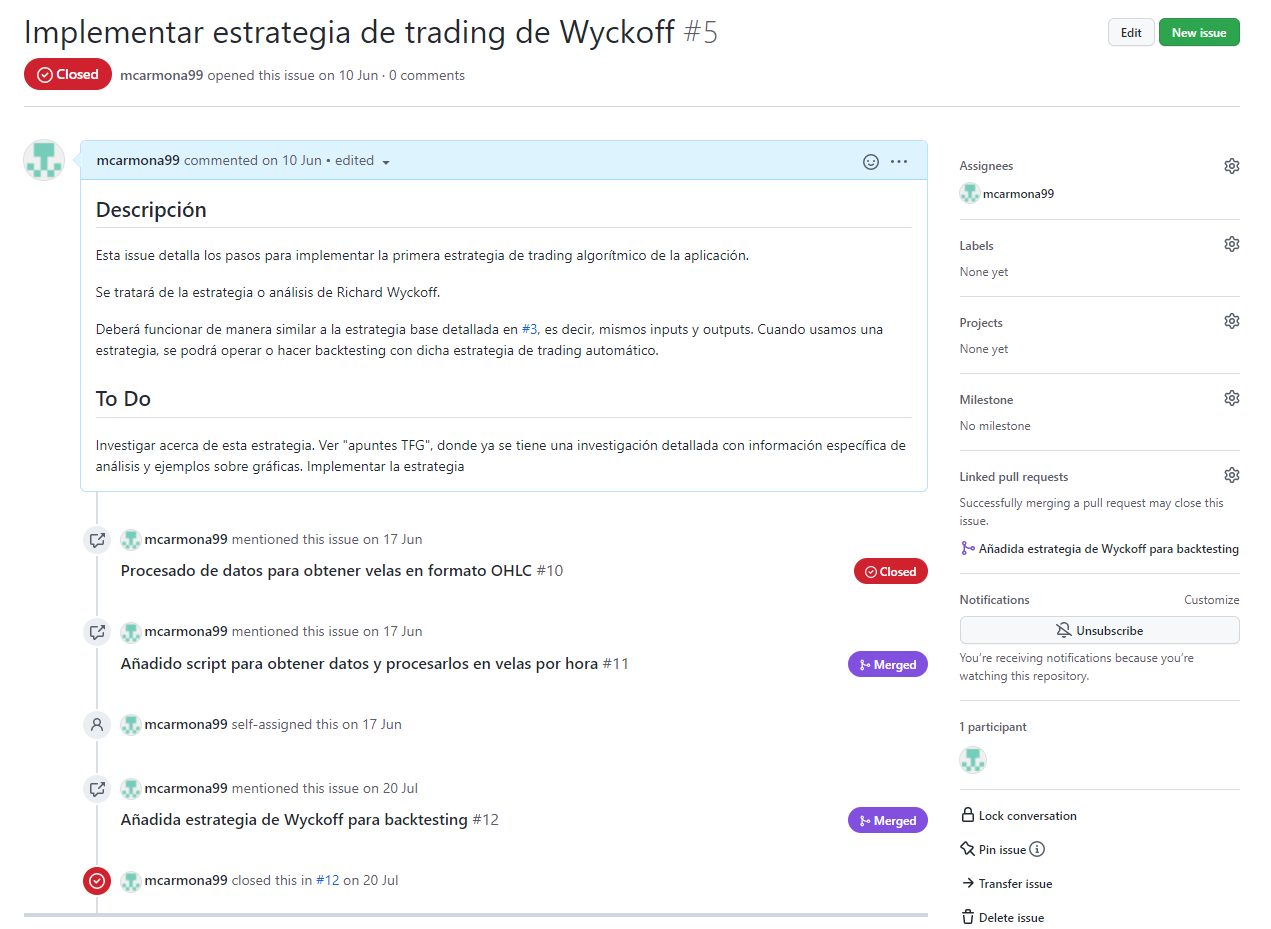
\includegraphics[width=1.2\textwidth]{imagenes/issue_pr/issue.png}
	\caption{\textit{Issue} número 5, implementación de la estrategia de Wyckoff} \label{issue}
\end{figure}

\begin{figure}[h]
	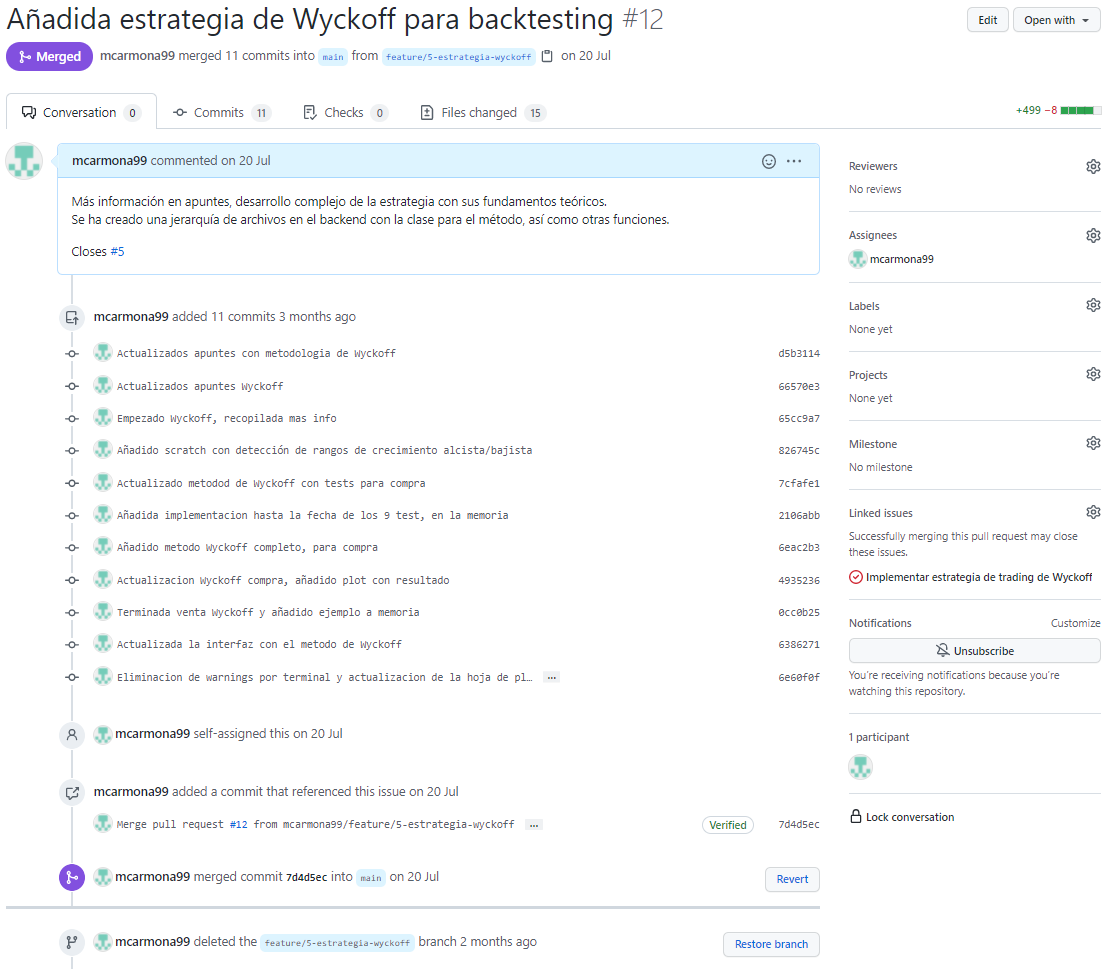
\includegraphics[width=1.2\textwidth]{imagenes/issue_pr/pr.png}
	\caption{\textit{Pull Request} referente a la issue \ref{issue}} \label{pr}
\end{figure}

\subsection{Paralelismo usando GitFlow}

\textit{GitFlow} es un flujo de trabajo basado en \textit{git} que brinda un mayor control y organización en el proceso de integración continua.\newline

El flujo de trabajo con GitFlow se basa principalmente en dos ramas; la rama \textit{develop} y la rama \textit{master}. La rama develop es aquella rama donde convergen las ramas de desarrollo. La rama master, en cambio, es la rama principal y estable (develop también es considerada estable). Esto puede variar en los desarrollos. En mi caso, \textit{main} es la rama que haría de \textit{develop} y a la que se incluyen los desarrollos.\newline

Los nuevos desarrollos parten de la rama develop y se mergean en ella misma una vez se han revisado. Dichos nuevos desarrollos son realizados en ramas que tienen nomenclaturas similares a:\newline

\begin{itemize}
	\item \textbf{feature/\#issue-descripcion-desarrollo}: rama que introduce una nueva funcionalidad.
	\item \textbf{fix/\#issue-descripcion-arreglo}: rama que introduce un fix a un bug o error conocido. En ocasiones tenemos hotfix o bugfix en lugar de fix.
	\item \textbf{support/\#issue-descripcion}: para soporte de pago o soporte a usuarios.
	\item \textbf{release/\#issue-descripcion}: para ramas de release.
\end{itemize}	

Cuando estos desarrollos han terminado, como hemos dicho anteriormente, sus ramas correspondientes son mergeadas a develop, por medio de un Pull Request. Lo normal es que cada PR esté asignado a una issue y a una rama.
\newline

Esto no ha sido de mucha utilidad en el caso de este proyecto, ya que no ha sido un trabajo en el grupo con lo que las ventajas de \textit{GitFlow} no se han visto en gran medida. \newline

\section{Fases del desarrollo}


\section{Diseño final de la interfax}


